% \documentclass[aspectratio=169,notes]{beamer}
\documentclass[aspectratio=169]{beamer}
\usetheme[faculty=phil]{fibeamer}
\usepackage{polyglossia}
\setmainlanguage{english} %% main locale instead of `english`, you
%% can typeset the presentation in either Czech or Slovak,
%% respectively.
\setotherlanguages{russian} %% The additional keys allow
%%
%%   \begin{otherlanguage}{czech}   ... \end{otherlanguage}
%%   \begin{otherlanguage}{slovak}  ... \end{otherlanguage}
%%
%% These macros specify information about the presentation
\title[Theoretical Mechanics]{Big HW 1} %% that will be typeset on the
\subtitle{ Particle kinematics \\
\  \\ \  \
         } %% title page.
\author{Oleg Bulichev}
%% These additional packages are used within the document:
\usepackage{ragged2e}  % `\justifying` text
\usepackage{booktabs}  % Tables
\usepackage{tabularx}
\usepackage{tikz}      % Diagrams
\usetikzlibrary{calc, shapes, backgrounds}
\usepackage{amsmath, amssymb}
\usepackage{url}       % `\url`s
\usepackage{listings}  % Code listings
% \usepackage{subfigure}
\usepackage{floatrow}
\usepackage{subcaption}
\usepackage{mathtools}
\usepackage{todonotes}
\usepackage{fontspec}
\usepackage{multicol}
\usepackage{pdfpages}
\usepackage{wrapfig}
\usepackage{animate}
\usepackage{booktabs}
\usepackage{multirow}
% \usepackage{graphicx}
\usepackage{colortbl}

\graphicspath{{resources/}}
\frenchspacing

\setbeamertemplate{caption}[numbered]
\usetikzlibrary{graphs}

% \usepackage[backend=biber,style=ieee,autocite=footnote]{biblatex}
% \addbibresource{biblio.bib}
% \DefineBibliographyStrings{english}{%
%   bibliography = {References},}

\newcommand{\oleg}[2][] {\todo[color=red, #1] {OLEG:\\ #2}}
\newcommand{\fbckg}[1]{\usebackgroundtemplate{\includegraphics[width=\paperwidth]{#1}}}%frame background

\usepackage[framemethod=TikZ]{mdframed}
\newcommand{\dbox}[1]{
\begin{mdframed}[roundcorner=3pt, backgroundcolor=yellow, linewidth=0]
\vspace{1mm}
{#1}
\vspace{1mm}
\end{mdframed}
}

\begin{document}
\setlength{\abovedisplayskip}{0pt}
\setlength{\belowdisplayskip}{0pt}
\setlength{\abovedisplayshortskip}{0pt}
\setlength{\belowdisplayshortskip}{0pt}

\fbckg{fibeamer/figs/title_page.png}
\frame[c]{\setcounter{framenumber}{0}
    \usebeamerfont{title}%
    \usebeamercolor[fg]{title}%
    \begin{minipage}[b][6.5\baselineskip][b]{\textwidth}%
        \textcolor{black}{\raggedright\inserttitle}
    \end{minipage}
    % \vskip-1.5\baselineskip

    \usebeamerfont{subtitle}%
    \usebeamercolor[fg]{framesubtitle}%
    \begin{minipage}[b][3\baselineskip][b]{\textwidth}
        \raggedright%
        \insertsubtitle%
    \end{minipage}
    \vskip.25\baselineskip
}
%   \frame[c]{\maketitle}

\fbckg{fibeamer/figs/common.png}

\begin{frame}[t]{Task description}
\framesubtitle{}
\vspace*{-0.4cm}
  \begin{columns}[T,onlytextwidth]
    \begin{column}{0.69\textwidth}
      \scriptsize
      We have a mobile vehicle, which should survive after the track. We have some predefined trajectory, which is given in $y(x)$ format. 
      \medskip

      The \textbf{goal} is to pass this trajectory as fast as possible. But at the end of the path, there is a drop-off. It means that the vehicle should stop in the end.
            \medskip
      
      We have to establish some constraints, such as max tangent acceleration (max power on the motor), normal acceleration (road adhesion).
      \medskip
      
      How the vehicle should move (speed and acceleration) for solving such a task?

      \textbf{Report}:
      \begin{enumerate}
        \item Vehicle simulation on the path. You should show a $\vec{v},\ \vec{a},\ \vec{a}_\tau,\ \vec{a}_n$ on the simulation.
        \item plots: $y(t),\ v(t),\ a_t(t), a_n(t)$, --- $t$ is time in seconds. 
      \end{enumerate}
      \textbf{Parameters}:\\
      $y(x) = Ax \ln (\dfrac{x}{B})$, where $A = 3,\ B = 5$, $x\in [0..4]$ \\
      $a_{t_{max}} = 2,\ a_{n_{max}} = 3,\ v_{max} = 3$
    \end{column}
    \begin{column}{0.29\textwidth}
      \begin{figure}[H]
        \centering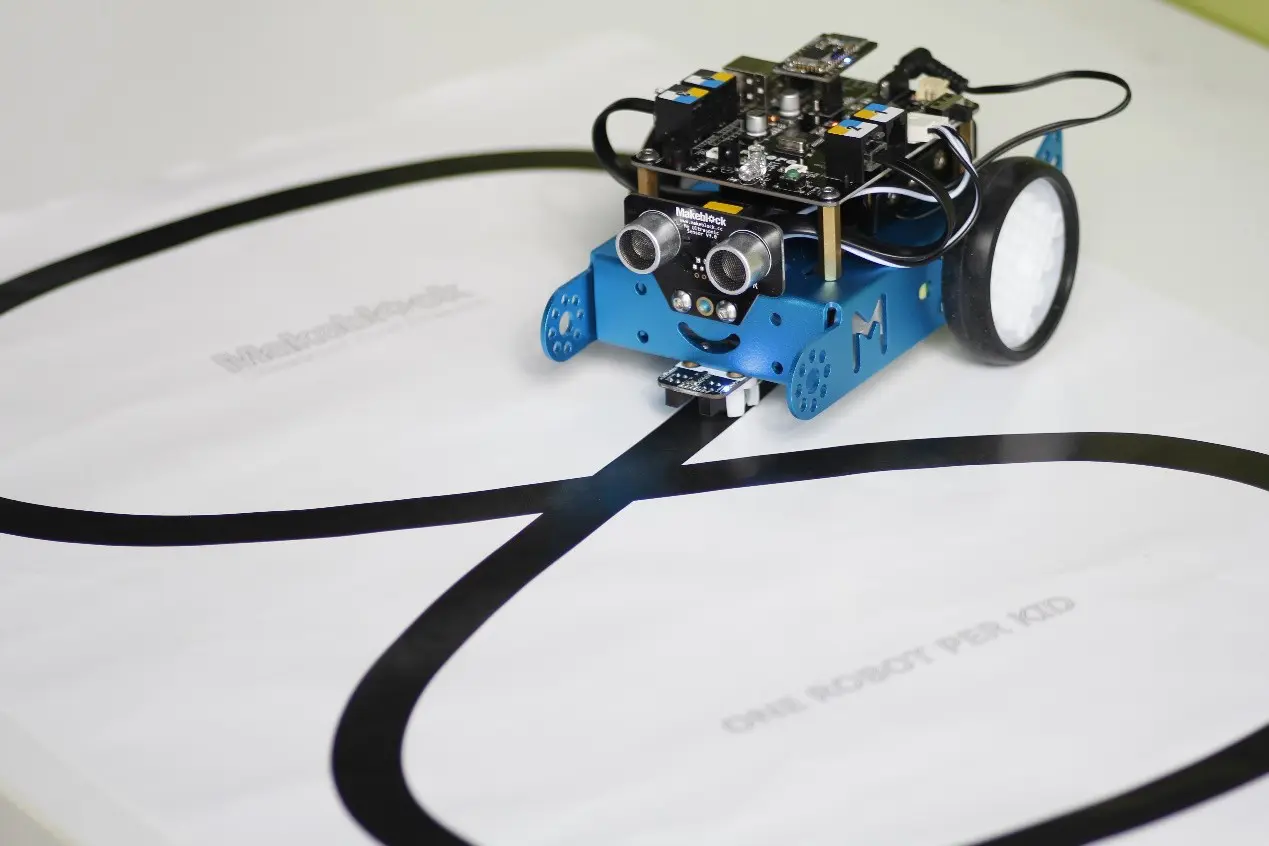
\includegraphics[height=6cm,width=1\textwidth,keepaspectratio]{picpic.png}
      \end{figure}
    \end{column}
  \end{columns}
\end{frame}

\begin{frame}[t]{Hints}
\framesubtitle{}
  \begin{itemize}
    \item Trapezoidal velocity and acceleration (subfolder <<extra material>>)
    \item Change between coordinate and natural forms (1st lab slides, theory)
    \item Curvature (1st Week HW)
    \item It's not a task about control. Your vehicle should move ideally along the trajectory.
  \end{itemize}
\end{frame}

\fbckg{fibeamer/figs/last_page.png}
\frame[plain]{}
\end{document}